\chapter{Analysis and hardening of a FPGA Design with a MicroBlaze}

A SRAM-based FPGA is sensitive to SEUs, as explained in Chapter \ref{sec:background}. To better understand the effects of radiation on the FPGA, it is better to see a design as an abstraction of two layers. The two main layers are:

\begin{itemize}
    \item \textit{Application layer}: includes the logic and memory elements as described by the user.
    \item \textit{Configuration layer}: includes the logic and memory elements that are used to implement physically the user's design in the FPGA.
\end{itemize}

From the logical point of view, a particle causing a SEU can affects one of the two layers, producing different consequences:

\begin{itemize}
    \item SEUs in the Application Layer manifest as transient errors that could affect the stored data or the state of the user logic memory elements such as BRAMs or Flip-Flops. 
    \item SEUs affecting the Configuration Layer manifest as persistent errors, that could be reverted using a reconfiguration process. 
\end{itemize}

The first one are transients because they are in the user logic and are directly controlled by the user. Because of that, they may be detected or corrected, it depends on how the logic has been designed. The second one are persistent because they directly affects how the bottom hardware works: from the point of view of the user, it is like a real hardware fault that cannot be corrected. \bigskip

Persistent errors can have two main consequences:

\begin{itemize}
    \item They can change a routing element connection or can complete disconnect internal wires.
    \item They can change the behaviour of a LUT.
\end{itemize}

SEUs in the configuration layer are the most common type of errors in SRAM-based FPGAs because the application layer virtually uses less area than the configuration layer. A summary of the different causes of SEUs is presented in the following table:

\begin{table}[H]
\centering
    \begin{tabular}{|cc|cp{6.2cm}|}
        \hline
        \textbf{Layer} & & \textbf{Element} & \textbf{SEU Consequence} \\
        \hline
        \multirow{12}{*}{Configuration}
        & & Muxes & Wrong input selection, open net, wrongly driven or left open\\
        \cline{3-4}
        & Routing & PIP & Wrong connection or disconnection between nets\\
        \cline{3-4}
        & & Buffers & Output net wrongly driven or left open\\
        \cline{2-4}
        & & LUT & Wrong function inputs and outputs \\
        \cline{3-4}
        & Logic & Control Bits & Wrong function inputs and outputs\\
        \cline{3-4}
        & & Tie Offs & Wrong function initialization\\
        \hline
        \multirow{2}{*}{Application}
        & & RAM Blocks & Wrong application data\\
        \cline{3-4}
        & & CLB Flip-Flops & Wrong application data or state\\
        \hline
    \end{tabular}
\caption{SEU consequences in SRAM-based FPGAs \cite{10.1145/1046192.1046212}}
\label{tab:conseq_fpgas_seu}
\end{table}

The following analyzes are focused on SEUs affecting the configuration layer, as they are the most common type of errors in SRAM-based FPGAs. However, the proposed techniques allows designeers to detect and correct SEUs in the application layer, too.

\section{How SEUs affect the MicroBlaze?}

As anticipated in the previous sections, the object of interest of this thesis work is the analysis of the MicroBlaze behaviour when affected by SEUs and how those effects can be mitigated by constructing a series of ad-hoc hardening technique. \bigskip

First, in order to understand how the MicroBlaze reacts to SEUs affecting itself, a series of fault injection campaign must be executed. The idea is to start with a very minimal hardware design that includes a MicroBlaze and a set of minimal peripherals. Thanks to the Block Design tool, the preparation of the design is very simple and straightforward, and the result is shown in Figure \ref{fig:base_mb}:

\begin{figure}[H]
\centering
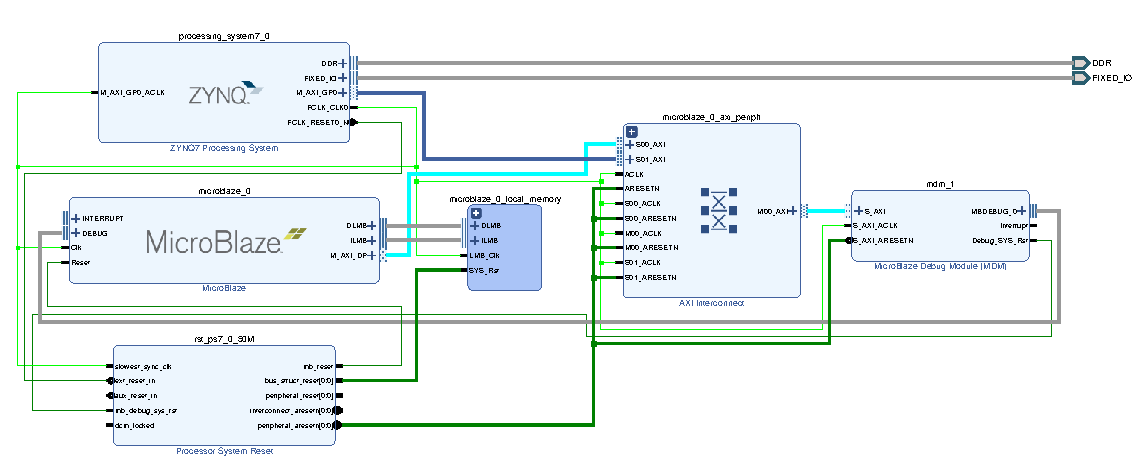
\includegraphics[width=1.0\linewidth]{images/chapter4/mb_base_design_edit.pdf}
\caption{Schematic of a basilar MicroBlaze design}
\label{fig:base_mb}
\end{figure}

In the schematic, the following blocks are present:
\begin{itemize}
    \item \textit{ZYNQ7 Processing System}: it represents the ZYNQ7020's Processing System (PS) from the point of view of the Programmable Logic (PL), as explained in Chapter \ref{sec:pynq}. It can offer a wide range of functionalities to the PL. For the moment, it is only used as a clock source and as a reset source. Via the ZYNQ7 PS block's configuration wizard, it is possible to configure a Phase-Locked Loop (PLL) in order to generate a clock for the PL with a specific frequency. For now, the PLL is configured to generate a clock for the PL with a frequency of 50 MHz, the same as the reference one given by the PYNQ-Z2 board.
    \item \textit{Processor System Reset}: is a soft IP that provides a mechanism to handle the reset conditions for a given system. The core handles numerous reset conditions at the input and generates appropriate resets at the output. For this simple design, the PSR is able to handle reset requests both from the PS and from the \textit{Debug Core}. It generates a active-high reset signal for the MicroBlaze core and for the Local Memory. Moreover, it generates a acthive-low reset signal for the AXI peripherals. 
    \item  \textit{MicroBlaze}: it represents the MicroBlaze instance under test. It has as inputs some debug signals from the Debug Core, the clock and the reset signal coming from the PSR. It offers as outputs the two memory buses for the Local Memory, one for the data memory (DLMB) and one for the instruction memory (ILMB). The last output is the AXI bus, which is used to access the peripherals through a \textit{AXI Interconnect}.
    \item \textit{Local Memory}: it is a sub-design (automatically generated by Vivado) that interfaces some BRAMs (a special kind of memory offered by the FPGA) with the Local Memory Bus (LMB). Block RAMs (or BRAMs) stands for Block Random Access Memory. Block RAMs are used for storing large amounts of data inside FPGAs.
    \item \textit{AXI Interconnect}: it is a sub-design (automatically generated by Vivado). As the name suggests, it is used to connect one or more AXI memory-mapped master devices to one or more memory-mapped slave devices.
    \item \textit{MicroBlaze Debug Module}: it is the Debug Core, and its main job is to enable JTAG-based software debugging of the MicroBlaze core. Moreover, it includes a configurable UART via an AXI interface. The UART's \textit{RX} and \textit{TX} signals are transmitted over the device JTAG port and can be accessed via the XSCT tool. With this setup, XSCT offers to designers the possibility to interact with the MicroBlaze core via a UART and to control the MicroBlaze core (status, registers, and software debug in general).
\end{itemize}

\begin{figure}[H]
\centering
\includegraphics[width=0.6\linewidth]{images/chapter4/hier.png}
\caption{Resulting hierarchy of the MicroBlaze design}
\label{fig:hier_mb}
\end{figure}

By looking at the schematic, there are two AXI masters connected to the AXI Interconnect. Hence, there are two different memory address spaces, and they are configured as follows:\bigskip

\begin{bytefield}{24}
    \begin{rightwordgroup}{/microblaze\_0}
        \memsection{0x4140\_0fff}{0x4140\_0000}{3}{4 KB MDM UART}\\
        \memsection{0x413f\_ffff}{0x0001\_0000}{3}{-- reserved --}\\
        \memsection{0x0000\_ffff}{0x0000\_0000}{6}{64 KB DLMB}
    \end{rightwordgroup}\\\\
    \begin{rightwordgroup}{/processing\_system7\_0}     
        \memsection{0x4140\_0fff}{0x4140\_0000}{3}{4 KB MDM UART}
    \end{rightwordgroup}
\end{bytefield}\bigskip

Finally, the design definition is ready and it can be synthesized and implemented. Because the aim of this design is to be analyzed by injecting faults, the MicroBlaze has been constrained to be placed in a specific portion of the FPGA, as explained in Chapter \ref{sec:fitollo}. This is possible with Vivado by defining a PBLOCK. \bigskip

A PBLOCK is a collection of cells, grouped in one rectangular area or region that specify the device resources contained by the PBLOCK. PBLOCKs are used during floorplanning. A design floorplan is broadly defined as a set of physical constraints used to control how the logic is placed into the FPGA. A good floorplan can help reduce routing congestion and improve the quality of timing results. On the other hand, a bad floorplan can reduce performances as well as unmet constraints if the required placement is unfeasible. \bigskip

As an example, the above design is implemented with the following constraints:

\begin{lstlisting}[style=tcl]
create_pblock pblock_1
add_cells_to_pblock [get_pblocks pblock_1] [
    get_cells -quiet [
        list design_1_i/microblaze_0
    ]
]

resize_pblock [get_pblocks pblock_1] -add {
    SLICE_X54Y102:SLICE_X67Y148
}

set_property IS_SOFT 0 [get_pblocks pblock_1]
\end{lstlisting}

In the above constraints, a PBLOCK called \textit{pblock\_1} is first defined. Than all the cells belonging to the Microblaze instance (\textit{design\_1\_i/microblaze\_0}) are added to the PBLOCK, and finally the PBLOCK is resized. The resize operation is used to define the physical resources that are included in the PBLOCK. As final operation, the PBLOCK is marked as a \textit{not soft} PBLOCK, which means that each MicroBlaze cell must be placed in that specific PBLOCK, and so it is a hard constraint.\bigskip

Once the constraints are ready, the design can be synthesized and implemented. The resulting floorplan is shown in the following figure:

\begin{figure}[H]
\centering
\includegraphics[width=0.7\linewidth]{images/chapter4/impl.png}
\caption{Resulting floorplan of the MicroBlaze design, with the PBLOCK on the top side. Microblaze cells are highlighted in red}
\end{figure}

Finally it is possible to launch the fault injection tool by providing the bitstream with no CRC and a .elf file to be executed by the MicroBlaze at each run. The resulting fault injection campaign is shown in the following:

\newpage
\begin{lstlisting}[style=preformatted]
Total injected bitflips = 12555

    --- FUNCTIONAL ANALYSIS ---
Correct results -> 11743 [93.53%]
Faulty results(SDE) -> 0 [0.0%]
MicroBlaze halted -> 744 [5.93%]
Total exceptions -> 68 [0.54%]

EXCEPTIONS:
 - XEXC_ID_FSL = 0 [0.0%]
 - XEXC_ID_UNALIGNED_ACCESS  = 19 [0.15%]
 - XEXC_ID_ILLEGAL_OPCODE  = 36 [0.29%]
 - XEXC_ID_M_AXI_I_EXCEPTION_or_XEXC_ID_IPLB_EXCEPTION = 0 [0.0%]
 - XEXC_ID_M_AXI_D_EXCEPTION_or_XEXC_ID_DPLB_EXCEPTION = 13 [0.1%]
 - XEXC_ID_DIV_BY_ZERO  = 0 [0.0%]
 - XEXC_ID_STACK_VIOLATION_or_XEXC_ID_MMU  = 0 [0.0%]
 - XEXC_ID_FPU  = 0 [0.0%]

\end{lstlisting}

% Explain here what are the effects of SEUs in the MicroBlaze.

\section{Strategies and adopted solutions}

% This section is focused on SEUs affecting the configuration layer, as they are more likely to occur. To overcome their effects, some techniques that exploit the particular reconfigurable capabilities of the FPGAs to detect and correct persistent errors in the configuration memory are detailed next:

% Scrubbing is a technique used to correct and prevent errors in the information stored in memory. In FPGAs, scrubbing can be used to mitigate both persistent errors in SRAM cells (i.e., the configuration memory) and transient errors in user-memory elements such as BRAMs. To perform configuration memory scrubbing, the configuration memory data must be read sequentially from the start to the end and compared to the original configuration bitstream or an error check code such as a cyclic redundancy check (CRC) [43].
% Dynamic partial reconfiguration allows run-time reconfiguration without application layer interruption. This technique cannot detect errors by itself, so it must be combined with other error detection techniques such as those based on redundancy. These correction techniques take advantage of the subdivision of the configuration memory into frames, which contain information related to the configuration of specific parts of the design.


Watchdog + DFX because..

\section{Development of a watchdog}

Beacon watchdog here

\subsection{What is a watchdog?}

A watchdog is ..

\subsection{How to implement a watchdog?}

Architecture of the watchdog (FSM)

\subsection{How to harden the watchdog?}

TMR.

\subsection{Integration of the watchdog in the design}

\section{How to partial reconfigure a design?}
\subsection{What is and how useful is a partial reconfiguration?}
\subsection{Xilinx DFX Controller}
\subsection{Prepare a design for partial reconfiguration}
\subsection{Prepare a design with a MicroBlaze for partial reconfiguration}

\section{Integration of the watchdog and the DFX}
\subsection{The needed hardware}
\subsection{DFX Decoupler: why?}

\section{A script to automatize the process}